\documentclass[a4paper, 12pt]{article}

%\usepackage{savetrees}
\usepackage{graphicx}
\usepackage{subfig}

%code for creating python code snippets
\usepackage{float}
\floatstyle{ruled}
\newfloat{python}{thp}{lop}
\floatname{python}{Listing}
%end code for creating python code snippets

\graphicspath{{./images/}}
\title {Student Robotics 2009\\ JointIO Board Documentation}
\date{\today}
\setcounter{tocdepth}{1}


\begin{document}

\maketitle

\noindent This document describes the functions of the JointIO Board. 

\begin{figure}
\centering
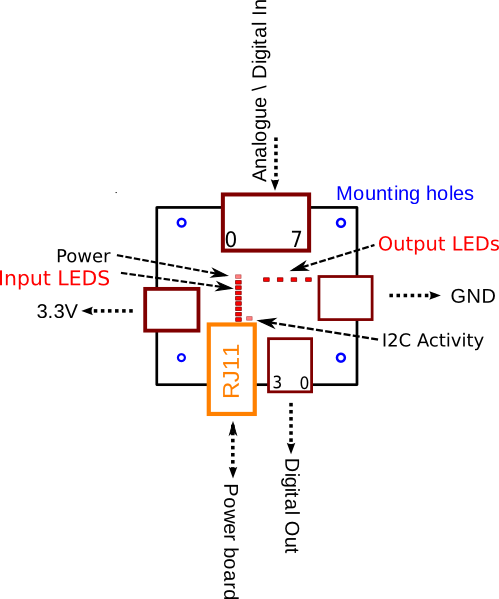
\includegraphics[scale=1, angle=0]{outline}
\caption{Jointio Board 1:1 Scale Drawing}
\label{fig:outline}
\end{figure}


\section{Board Outline}
Figure \label{fig:outline} is a 1:1 scale drawing of the Joint Input/Output board which can be printed out and used to aid drilling holes for mounting.
\label{sec:outline}

\section{Brief Description}

The Joint Input/Output (herein referred to as JointIO) provides analogue inputs and digital outputs for use on your robot.  

For instructions on how to assemble the JointIO board and Student Robotics kit, see \textit{Student Robotics Assembly Guide 2009}, available from the website.


\section{Cage Clamps}
Connections are made to the JointIO Board using the green and orange cage clamps which surround the board. These provide a solder-less, secure connection - requiring only a screwdriver or small fingers. 
\newpage

\section{Inputs}
Eight analogue inputs are provided by the JointIO Board. These are labelled 0 to 7 and can be treated as \textbf{digital} inputs in your code if desired. Power and ground connections are provided to enable switches and external circuits to be interfaced. Figure \ref{fig:analogue-in} demonstrates how a rotary potentiometer can be connected to the JointIO board to measure the angular rotation of an armature. Figure \ref{fig:digital-in} shows how a simple bump switch may be configured.

Note: The analogue readings of the input pin assume that the input voltage range is between GND and 3.3V. 

The logic value of these input pins are echoed onto the input LEDs on the board. This gives a visual indication of which inputs are high/low.

\begin{figure}[h]
\centering
\subfloat[Example analogue input configuration]{\label{fig:analogue-in}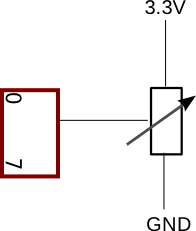
\includegraphics[scale=0.6, angle=0]{analogue-in}}
\hspace{60pt}
\subfloat[Example digital bump switch input configuration]{\label{fig:digital-in}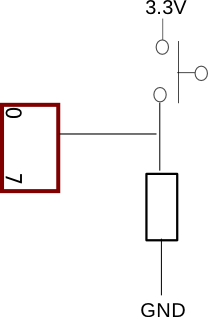
\includegraphics[scale=0.6, angle=0]{digital-in}}
\caption{Example Input configurations}
\label{fig:inputs}
\end{figure}


\begin{python}
\begin{verbatim}

	io.pin(2) 		%returns bees 

\end{verbatim}
  \caption{Reading the value of io input pins} 
\end{python}


\section{Outputs}
Four digital outputs are provided by the JointIO Board. These are labelled 0 to 3 and may be used to trigger relays, LEDs, external logic circuits or anything else requiring a digital input. 

Note: The digital output pins will be at 3.3V (Logic 1) and GND (Logic 0)


The logic value of these output pins are echoed onto the output LEDs on the board. This gives a visual indication of which outputs are high/low.

\begin{python}
\begin{verbatim}

	io.pin(1) = 1		%set io pin 

\end{verbatim}
  \caption{Setting the value of io output pins} 
\end{python}

\section{Troubleshooting}
\subsection{Random input readings}
Do you have a common ground between the JointIO board and your external circuit providing the input? - If not the input value will appear to be floating!


\end {document}
